% Contributors: Kevin Wu, Emily Jin
\section{The \emph{k}-means problem}
The $k$-means optimization problem is defined as:
\begin{enumerate}
\item \underline{Input}: A set of $n$ points $\mathcal{S} = x_1,....x_n \in
\mathbb{R}^d$ and a positive integer $k<n$.
\item \underline{Output}: $T \subset  \mathbb{R}^d$ s.t. $|T|=k$. 
\item \underline{Goal}: minimize ``cost'' of $T$ where: $cost(T) 
:= \sum_{i = 1}^{n} \min_{\mu_j \in T} \norm{x_i-\mu_j}^2 $.
\end{enumerate}

Note that unlike the $k$-centers or $k$-medians problem, the $k$-means problem (as defined above) requires that the set of input points belong to a \emph{Euclidean} space as opposed to a metric space; later we will define a generalized $k$-means problem setup for which $x_1,....x_n$ may come from any metric space. \\

\noindent\textbf{Approximate solutions for $k$-means:}  

As before, we can attempt an exhaustive search with exponential
time complexity. If we want some solution in polynomial time, however, we
must settle for an approximation, as $k$-means is also an NP-hard
optimization problem. \\

(The statement regarding NP-hardness of $k$-means assumes that $d$ in $\mathbb{R}^d$ must be greater than or equal to 2; when $d = 1$, the problem is actually solvable in polynomial time using dynamic programming).\\

One approximate solution is Lloyd's method for $k$-means, which alternates between optimizing cluster assignments and cluster centers until some stopping criterion (i.e. convergence of cluster centers $\vec{\mu}$).

\begin{algorithm}
\caption{Lloyd's Algorithm:}
\begin{algorithmic} 
\STATE Pick randomly $x_1,...,x_k $ from $\mathcal{X}$ \;
\WHILE{stopping criteria not satisfied}
\STATE Assign points of the dataset to the closest center \;
\FORALL {clusters $C_1, ..., C_k$\;}
\STATE Compute the new centroid $\mu_j = \frac{1}{|C_j|}
\sum_{x_i\in C_j} x_i$, $\forall j \in \{1,...,k\}$\;
\ENDFOR
\ENDWHILE
\end{algorithmic}
\end{algorithm}

\begin{remark}
Call $cost(T^*)$ the cost of the optimal k-means solution, and $cost(T^{LLOYD})$ the cost the approximate solution returned by k-means. Then necessarily, $cost(T^{LLOYD}) \geq cost(T^*)$.
\end{remark}

\begin{remark}
$cost(T^{LLOYD})$ is unbounded and may be \emph{arbitrarily bad} compared to the optimal solution depending on the initialization of cluster means.
\end{remark}

\begin{example} 
Llyod's method is arbitrarily bad even for seemingly ideal inputs. Consider data that is actually separable into $k=3$ collinear clusters, the diameter of each of which is $\delta$. Let the distance between the middle cluster and the other two clusters be $\Delta$, and let $n$ be the number of points in each cluster, for $3n$ points total. 

\begin{figure}
	\centering
	\captionsetup{width=0.8\textwidth}
	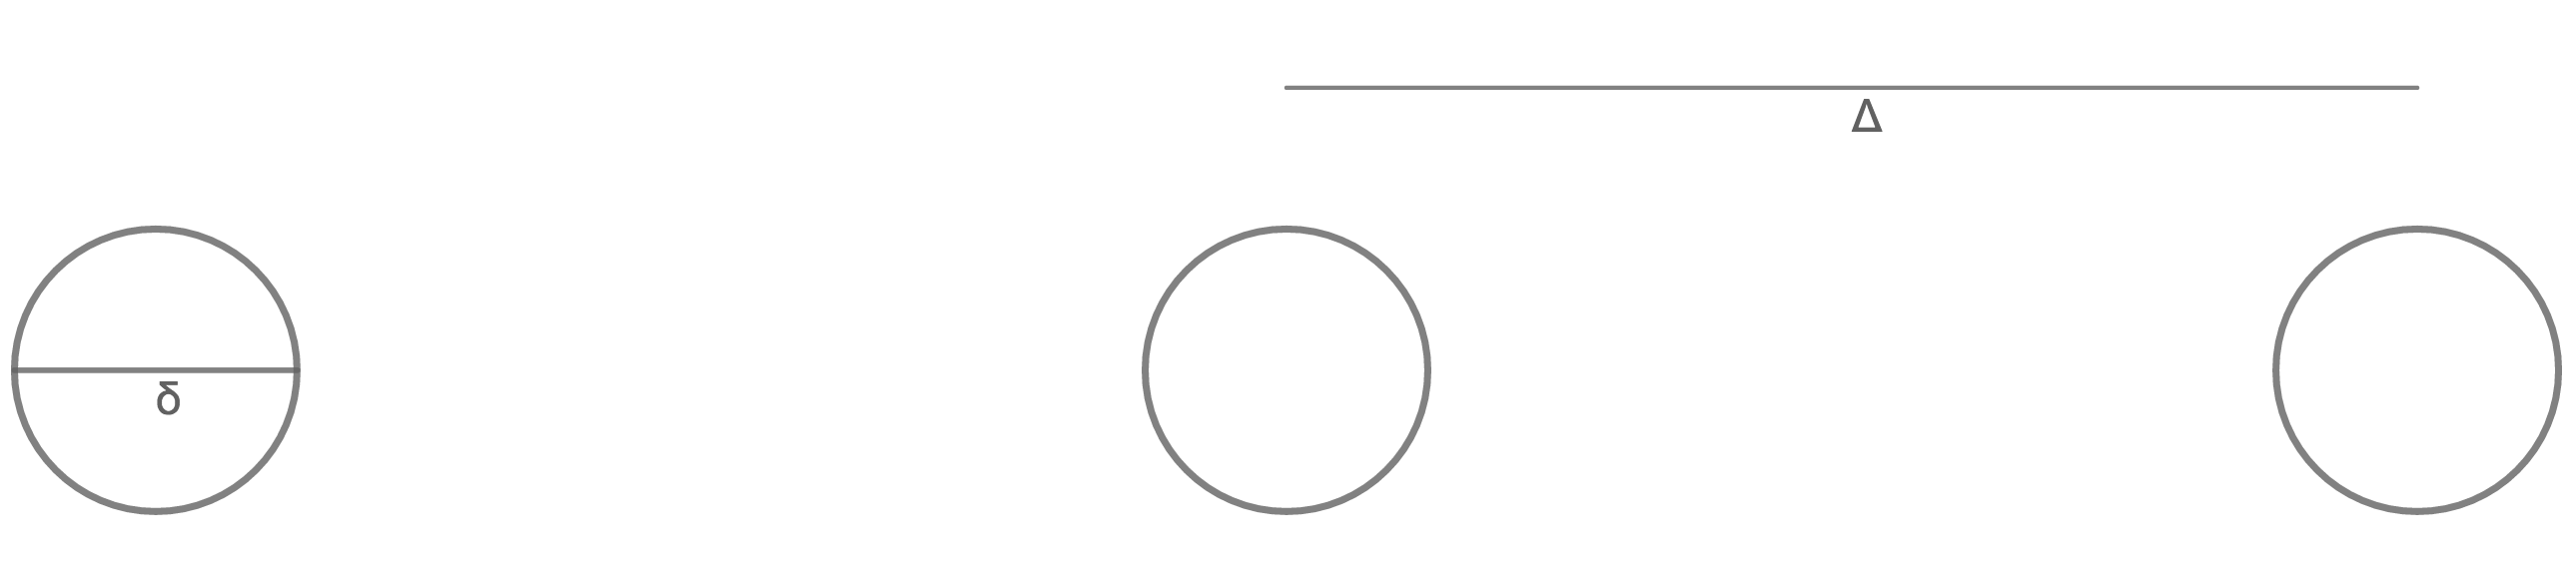
\includegraphics[scale=0.6]{chapter_1/files/kmeans.png}
	\caption{An example of a "nice" set of clusters for which Llyod's method can be arbitrarily bad.}
	\label{fig:kmeans}
\end{figure}

Llyod's method is given $k=3$ as part of its input and initializes its
cluster centers to be random data points. Suppose two of the initial
centers end up in the right cluster, and the third initial center is
in the middle cluster. Then all the points in the left and middle
clusters are assigned to the center that was initialized in the middle
cluster. When the center is updated to be the mean of all these
points, it moves to be between the left and the center clusters, which
is a stable configuration. 

\begin{figure}
	\centering
	\captionsetup{width=0.8\textwidth}
	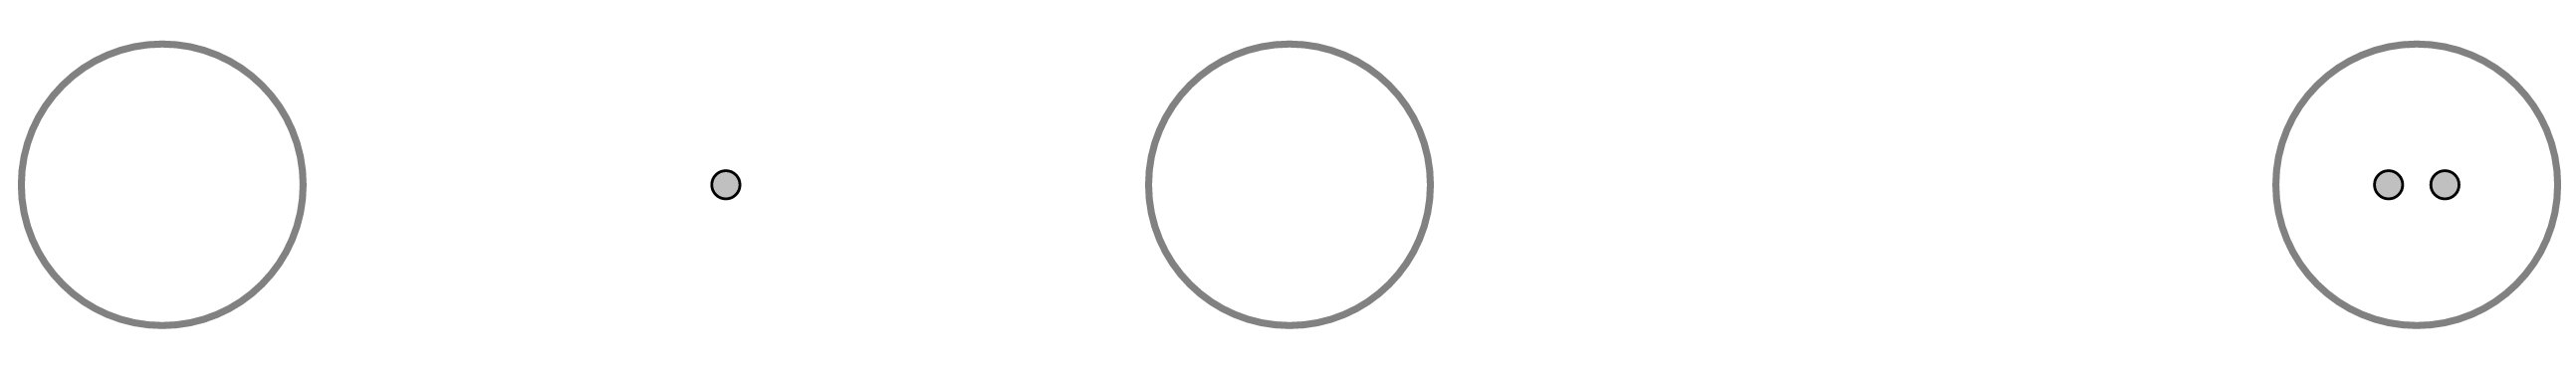
\includegraphics[scale=0.6]{chapter_1/files/stable-kmeans.png}
	\caption{A stable configuration with cost $\Omega(n\Delta^2)$.}
	\label{fig:kmeans}
\end{figure}

Consider the cost of this configuration. Because one of the centers is
between two clusters, and because the k-means cost is the sum of the
squared distances to each point's center, the total cost is
$\Omega(n\Delta^2)$. In contrast, the minimum cost (which is achieved
when the centers are initialized to be in separate clusters) is
$O(n\delta^2)$ since each points is within $O(\delta)$ of its center.
$\delta$ and $\Delta$ were arbitrary, so the bad case is arbitrarily
worse than the good case.
\end{example}




